\documentclass[12pt,a4paper]{article}
\usepackage{fontspec}\usepackage{polyglossia}\setdefaultlanguage{ukrainian}
\setmainfont{NewComputerModern10}\setsansfont{Noto Sans}\setmonofont{Noto Sans Mono}[Scale=.82]
\usepackage{amsmath,amssymb,booktabs,caption,enumitem,float,geometry,graphicx,hyperref,microtype,titlesec,xcolor}
\geometry{left=2cm,right=2cm,top=2cm,bottom=2cm}\setlength{\parindent}{1.25cm}\linespread{1.08}
\titleformat{\section}{\normalfont\fontsize{14}{16}\selectfont\bfseries}{\thesection}{.6em}{}\titlespacing*{\section}{0pt}{1.3em}{.6em}
\titleformat{\subsection}{\normalfont\fontsize{12}{14}\selectfont\bfseries}{\thesubsection}{.6em}{}
\captionsetup{font=small,labelfont=bf,labelsep=endash}
\usepackage[newfloat]{minted}\SetupFloatingEnvironment{listing}{name=Лістинг}
\setminted{fontsize=\footnotesize,linenos,breaklines,autogobble,frame=single,framesep=2mm,bgcolor=gray!5,tabsize=4}
\hypersetup{unicode,colorlinks=true,linkcolor=black,pdftitle={ІО-41, Давидчук А. М., Лабораторна робота №5},pdfauthor={Давидчук А. М.}}
\newcommand{\resultDir}{../results}\newcommand{\studentGroup}{ІО-41}\newcommand{\studentName}{Давидчук А. М.}\newcommand{\reportYear}{2026}
\begin{document}\pagenumbering{gobble}
\begin{titlepage}
\begin{center}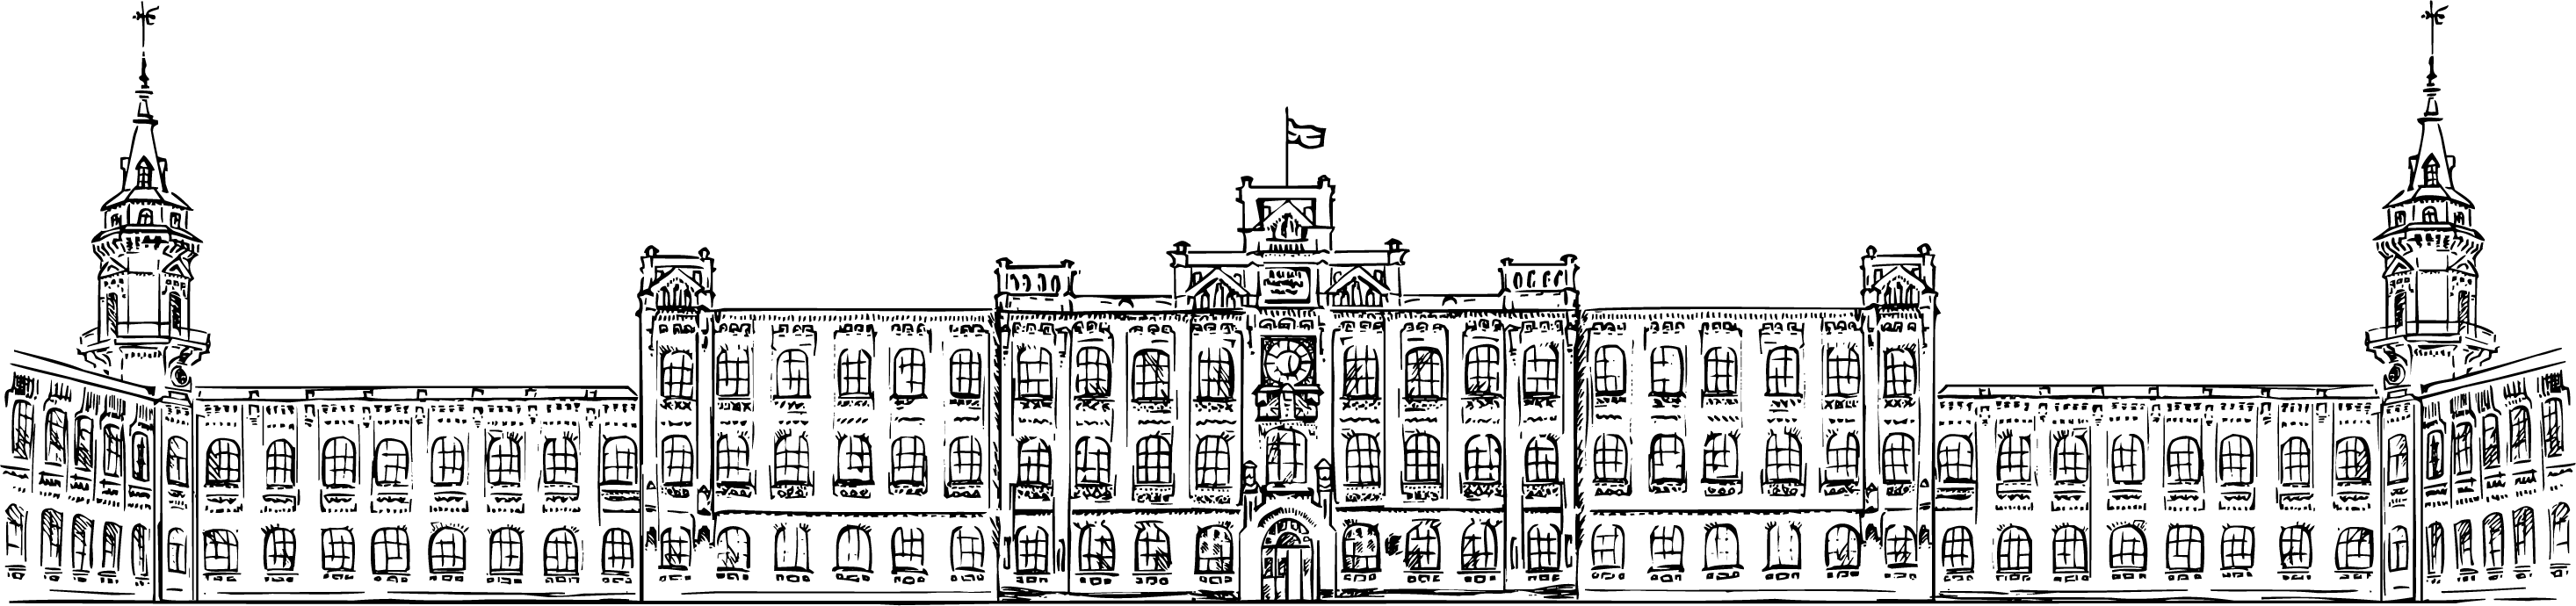
\includegraphics[width=.7\textwidth]{../../../../../../templates/letterhead.png}\end{center}
\begin{center}\large Національний технічний університет України\\ «Київський політехнічний інститут імені Ігоря Сікорського»\\[1em]Факультет інформатики та обчислювальної техніки\\Кафедра обчислювальної техніки\end{center}
\vfill\begin{center}\textbf{\LARGE Методи та технології штучного інтелекту}\\[2em]\textbf{\Large Лабораторна робота №5}\\[.7em]«Моделювання згорткової нейронної мережі»\end{center}
\vfill\begin{flushright}\begin{minipage}{.48\textwidth}Виконав: студент 3 курсу ФІОТ,\\групи \studentGroup\\\textit{\studentName}\\[1em]Перевірив: \textit{Польшакова О. М.}\end{minipage}\end{flushright}
\vfill\begin{center}Київ --- \reportYear\end{center}
\end{titlepage}\pagenumbering{arabic}

\section{Тема та мета роботи}
\noindent\textbf{Тема:} моделювання згорткової нейронної мережі для розпізнавання рукописних цифр.\\
\noindent\textbf{Мета:} дослідити принцип роботи згортки, підвибірки та повнозв'язного класифікатора; навчити CNN розпізнавати цифри MNIST і перевірити її стійкість до шуму та часткового пошкодження зображень.

\section{Постановка задачі та дані}
Потрібно побудувати програму, яка приймає монохромне зображення цифри розміром $28\times28$ пікселів і повертає один із десяти класів від 0 до 9. Для експерименту використано офіційний набір MNIST. Щоб обчислення залишалися відтворюваними і не потребували потужного GPU, з нього збалансовано відібрано 1500 навчальних і 300 тестових зображень: однакова кількість прикладів кожної цифри.

Пікселі переведено з діапазону $[0;255]$ у $[0;1]$. Окрему копію тестової вибірки спотворено гаусовим шумом; для частини зображень додано вузьке стирання. Чиста вибірка перевіряє базову точність, а пошкоджена --- стійкість моделі до помилок введення.

\section{Теоретичні відомості}
Згорткова нейронна мережа враховує просторову структуру зображення. Фільтр $K$ невеликого розміру послідовно переміщується по зображенню $X$, а елемент карти ознак обчислюється як
\begin{equation}S_{i,j}=\sum_{u=0}^{h-1}\sum_{v=0}^{w-1}X_{i+u,j+v}K_{u,v}+b.\end{equation}
Один фільтр може реагувати на край, штрих або інший локальний фрагмент. Однакові ваги застосовуються в усіх позиціях, тому згортка має значно менше параметрів, ніж повнозв'язний шар для всіх пікселів.

Після згортки застосовується ReLU: $\operatorname{ReLU}(x)=\max(0,x)$. Вона залишає додатні активації та додає нелінійність. Підвибірка $2\times2$ зменшує просторовий розмір карти ознак, скорочує кількість обчислень і робить ознаки менш чутливими до малих зміщень.

Вихідний повнозв'язний шар формує десять оцінок. Softmax перетворює їх на ймовірності:
\begin{equation}p_k=\frac{e^{a_k}}{\sum_{j=0}^{9}e^{a_j}}.\end{equation}
Навчання мінімізує перехресну ентропію $L=-\frac1n\sum_i\log p_{y_i}$. Градієнти обчислюються зворотним поширенням помилки, після чого ваги коригуються градієнтним спуском.

\section{Архітектура і параметри навчання}
Реалізована мережа має послідовність:
\begin{center}\texttt{28x28 → Conv(8 фільтрів, 5x5) → ReLU → AvgPool(2x2) → Dense(10) → Softmax}.\end{center}
Після згортки без доповнення отримується 8 карт $24\times24$, після підвибірки --- 8 карт $12\times12$. Вони розгортаються у вектор із 1152 ознак. Мережа навчається 20 епох пакетами по 50 зображень; початкова швидкість навчання становить 0,035 і поступово зменшується. Фіксований seed 4106 забезпечує повторюваність результатів.

\section{Програмна реалізація}
Згортка виконується векторизовано: спочатку формується представлення всіх вікон $5\times5$, потім вони множаться на вісім фільтрів. Основний прямий прохід наведено в лістингу.
\begin{listing}[H]
\inputminted[firstline=143,lastline=154]{python}{../src/main.py}
\caption{Пряме поширення сигналу в CNN}
\end{listing}

Під час навчання обчислюються градієнти вихідного шару, підвибірки та згорткових фільтрів. Це означає, що ядра не задаються вручну, а підлаштовуються за навчальними прикладами.
\begin{listing}[H]
\inputminted[firstline=156,lastline=178]{python}{../src/main.py}
\caption{Один крок зворотного поширення помилки}
\end{listing}

\section{Результати}
\begin{table}[H]\centering
\begin{tabular}{lr}\toprule Показник & Значення\\\midrule
Навчальних зображень & 1500\\
Тестових зображень & 300\\
Кількість епох & 20\\
Точність на чистих зображеннях & 88,67\%\\
Точність на пошкоджених зображеннях & 82,67\%\\
Фінальна навчальна втрата & 0,2337\\\bottomrule
\end{tabular}\caption{Результати навчання CNN}\end{table}

\begin{figure}[H]\centering\includegraphics[width=.9\textwidth]{\resultDir/training.png}\caption{Зміна функції втрат і точності під час навчання}\end{figure}
Крива втрат зменшується, а точність зростає, отже корекція фільтрів і ваг проходить у правильному напрямку. Різниця між чистою та пошкодженою вибірками становить 6 відсоткових пунктів. Модель зберігає працездатність при шумі, але найбільше помиляється на сильно деформованих цифрах зі схожими контурами.

\begin{figure}[H]\centering\includegraphics[width=.72\textwidth]{\resultDir/confusion_matrix.png}\caption{Матриця помилок на чистій тестовій вибірці}\end{figure}
Діагональні елементи матриці відповідають правильним прогнозам. Позадіагональні значення показують конкретні пари класів, які мережа плутає. Такий аналіз корисніший за одну загальну точність, бо дозволяє визначити проблемні цифри.

\begin{figure}[H]\centering\includegraphics[width=\textwidth]{\resultDir/clean_predictions.png}\caption{Розпізнавання чистих навчальних зображень MNIST}\end{figure}
Над кожним зображенням указано правильний клас і прогноз мережі. Цей рисунок безпосередньо демонструє працездатність CNN на прикладах із навчальної вибірки.

\begin{figure}[H]\centering\includegraphics[width=\textwidth]{\resultDir/predictions.png}\caption{Приклади розпізнавання зашумлених і частково стертих цифр}\end{figure}
Зеленим підписано правильні прогнози, червоним --- помилки. Навіть за наявності шуму більшість характерних штрихів зберігається, тому згорткові фільтри знаходять потрібні локальні ознаки.

\section{Висновки}
Реалізовано CNN без використання готового фреймворку глибокого навчання. Мережа самостійно навчає вісім згорткових фільтрів і класифікує цифри MNIST. На 300 чистих тестових зображеннях отримано точність 88,67\%, а після додавання шуму та стирань --- 82,67\%. Результат підтверджує, що згортка ефективно виділяє локальні ознаки, а підвибірка зменшує розмірність і частково підвищує стійкість до спотворень.

\section{Контрольні питання}
\begin{enumerate}[leftmargin=*]
\item \textit{Що таке згорткова нейронна мережа і для яких задач вона використовується?}\\
CNN --- мережа, що виділяє локальні просторові ознаки згортковими фільтрами. Її застосовують для класифікації, детекції та сегментації зображень.
\item \textit{Чим CNN відрізняється від повнозв'язної мережі?}\\
CNN використовує локальні зв'язки та спільні ваги фільтра, тому має менше параметрів і зберігає інформацію про взаємне розташування пікселів.
\item \textit{Що таке згортка?}\\
Це послідовне множення локального фрагмента входу на ядро з подальшим сумуванням, результатом якого є карта ознак.
\item \textit{Яку роль виконують фільтри?}\\
Фільтри навчаються реагувати на характерні локальні структури: краї, кути, дуги та складніші комбінації штрихів.
\item \textit{Що таке карта ознак?}\\
Це двовимірний масив активацій одного фільтра в різних позиціях зображення.
\item \textit{Для чого потрібен pooling?}\\
Він зменшує просторовий розмір карт, прискорює обчислення і знижує чутливість до невеликих зміщень.
\item \textit{Чим max pooling відрізняється від average pooling?}\\
Max pooling залишає найбільшу активацію у вікні, а average pooling обчислює середнє значення. У роботі використано усереднення.
\item \textit{Що таке padding і stride?}\\
Padding додає рамку навколо входу, а stride задає крок переміщення ядра.
\item \textit{Як padding і stride впливають на розмір виходу?}\\
Більший stride зменшує вихід, а padding може зберегти його розмір і дозволити обробляти крайові пікселі.
\item \textit{Які основні шари використовують у CNN?}\\
Згорткові, активаційні, pooling, нормалізаційні, повнозв'язні та вихідні шари.
\item \textit{Що таке перенавчання?}\\
Це ситуація, коли модель добре запам'ятала навчальні приклади, але гірше працює на нових даних.
\item \textit{Як зменшити перенавчання CNN?}\\
Застосовують dropout, регуляризацію ваг, аугментацію даних, ранню зупинку та збільшення навчальної вибірки.
\item \textit{Чому CNN ефективні для зображень?}\\
Вони використовують локальність, спільні ваги та ієрархічне виділення ознак від простих штрихів до цілих об'єктів.
\item \textit{Де, крім комп'ютерного зору, застосовують CNN?}\\
Для аналізу аудіо, часових рядів, сигналів датчиків і текстових послідовностей.
\item \textit{Які головні недоліки CNN?}\\
Для високої точності вони потребують багато даних і обчислень; результат роботи окремих фільтрів не завжди легко інтерпретувати.
\end{enumerate}
\end{document}
